% Original vector reconstruction of source Fig.26.1, PDF114.
% The gray disk is the hard connected block, not a bare four-point vertex.
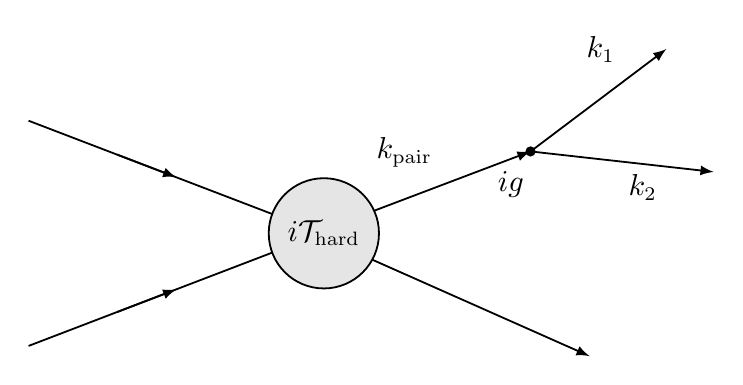
\begin{tikzpicture}[x=15mm,y=13mm,line width=.65pt,>=latex,
font=\fontsize{10.5}{12}\selectfont]
\draw (-2.5,1.1)--(-.35,.15);
\draw (-2.5,-1.1)--(-.35,-.15);
\draw[->] (-1.75,.769)--(-1.25,.548);
\draw[->] (-1.75,-.769)--(-1.25,-.548);
\draw[->] (.2,-.15)--(2.25,-1.2);
\draw[->] (.15,.1)--(1.75,.8);
\draw[->] (1.75,.8)--(2.9,1.8);
\draw[->] (1.75,.8)--(3.3,.6);
\node[circle,draw,fill=gray!20,minimum size=14mm,inner sep=1pt] at (0,0) {$i\mathcal T_{\rm hard}$};
\fill (1.75,.8) circle[radius=.65mm];
\node[above left] at (1,.55) {$k_{\rm pair}$};
\node[above left] at (2.55,1.57) {$k_1$};
\node[below] at (2.7,.67) {$k_2$};
\node[below left] at (1.78,.7) {$ig$};
\end{tikzpicture}
